%
%
%
%Appendix
%
%

\appendix

\section{Appendix}
\label{ch:appendix}

\subsection{User groups}
\label{sec:user_groups}

A detailed list of all examined Twitter accounts is omitted here for the sake
of brevity.
User groups were assembled as Twitter lists in the author's profile.
Find links to all lists in the following:

\begin{enumerate}
\item Celebrity user group: \url{https://twitter.com/_fpeters/lists/celebrities}
\item Politician user group: \url{https://twitter.com/_fpeters/lists/us-politicians}
\item Company user group: \url{https://twitter.com/_fpeters/lists/fortune-500}
\end{enumerate}

\subsection{Confusion matrices}
\label{sec:confusion_matrices}

Confusion matrices for favorite classification were omitted in the results chapter.
They are displayed in the following.

\begin{figure}[h]
\begin{subfigure}{.4\textwidth}
  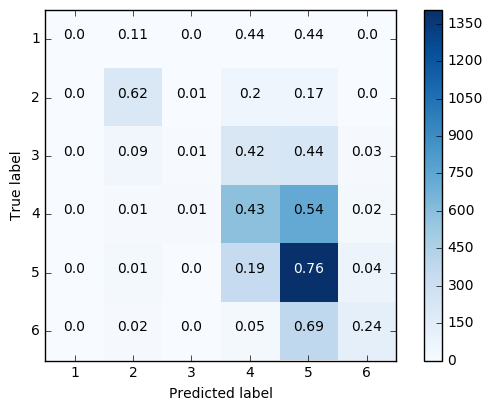
\includegraphics[width=.95\linewidth]{img/celeb_lin_cm_favorites}
  \caption{Celebrity data set}
  \label{fig:lin_fav_distr_sub1}
\end{subfigure}%
\begin{subfigure}{.4\textwidth}
  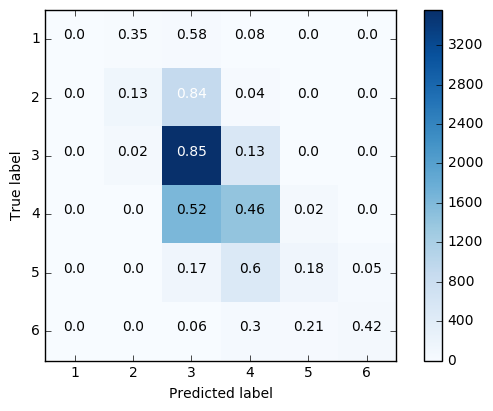
\includegraphics[width=.95\linewidth]{img/polit_lin_cm_favorites}
  \caption{Politician data set}
  \label{fig:lin_fav_distr_sub2}
\end{subfigure}
\begin{subfigure}{.4\textwidth}
  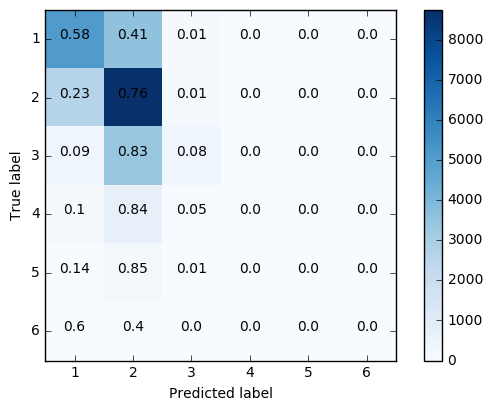
\includegraphics[width=.95\linewidth]{img/corp_lin_cm_favorites}
  \caption{Company data set}
  \label{fig:lin_fav_distr_sub3}
\end{subfigure}%
\begin{subfigure}{.4\textwidth}
  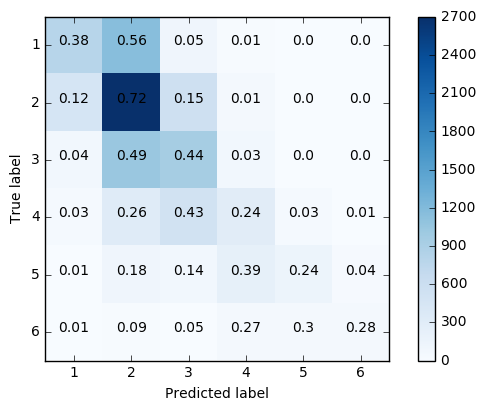
\includegraphics[width=.95\linewidth]{img/comb_lin_cm_favorites}
  \caption{Combined data set}
  \label{fig:lin_fav_distr_sub3}
\end{subfigure}%
\caption{Confusion matrices for linear retweet classification models}
\label{fig:lin_fav_cm}
\end{figure}

\begin{figure}[h]
\begin{subfigure}{.4\textwidth}
  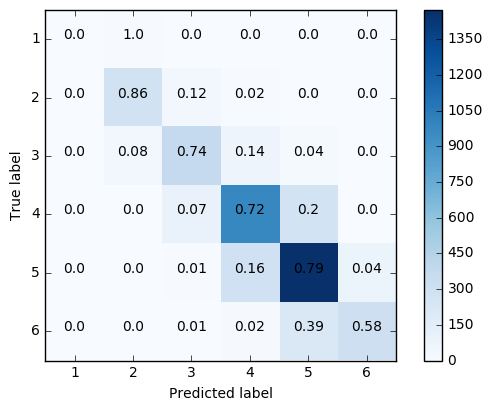
\includegraphics[width=.95\linewidth]{img/celeb_d1_cm_favorites}
  \caption{Celebrity data set}
  \label{fig:d1_fav_distr_sub1}
\end{subfigure}%
\begin{subfigure}{.4\textwidth}
  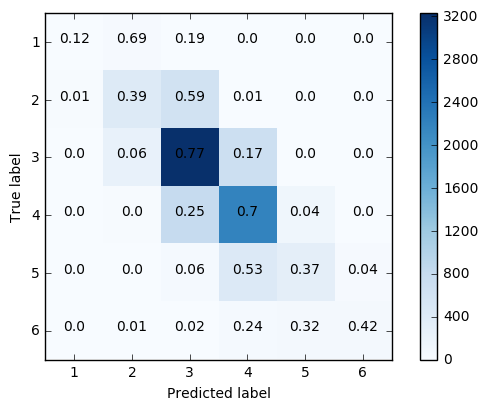
\includegraphics[width=.95\linewidth]{img/polit_d1_cm_favorites}
  \caption{Politician data set}
  \label{fig:d1_fav_distr_sub2}
\end{subfigure}
\begin{subfigure}{.4\textwidth}
  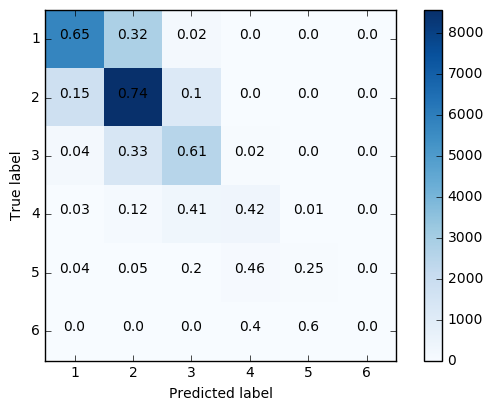
\includegraphics[width=.95\linewidth]{img/corp_d1_cm_favorites}
  \caption{Company data set}
  \label{fig:d1_fav_distr_sub3}
\end{subfigure}%
\begin{subfigure}{.4\textwidth}
  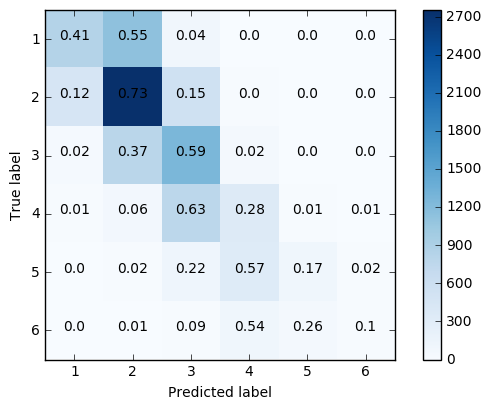
\includegraphics[width=.95\linewidth]{img/comb_d1_cm_favorites}
  \caption{Combined data set}
  \label{fig:d1_fav_distr_sub4}
\end{subfigure}%
\caption{Confusion matrices for deep feedforward classification models}
\label{fig:d1_fav_cm}
\end{figure}

\begin{figure}[h]
\begin{subfigure}{.4\textwidth}
  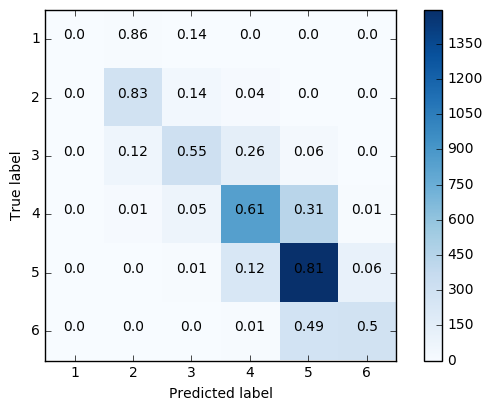
\includegraphics[width=.95\linewidth]{img/celeb_d2_cm_favorites}
  \caption{Celebrity data set}
  \label{fig:d2_fav_distr_sub1}
\end{subfigure}%
\begin{subfigure}{.4\textwidth}
  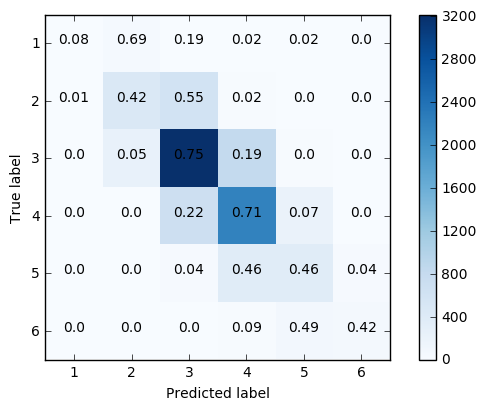
\includegraphics[width=.95\linewidth]{img/polit_d2_cm_favorites}
  \caption{Politician data set}
  \label{fig:d2_fav_distr_sub2}
\end{subfigure}
\begin{subfigure}{.4\textwidth}
  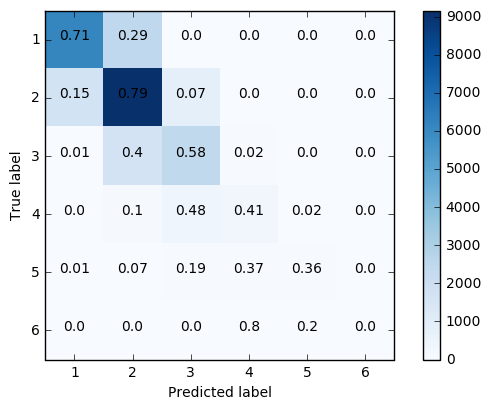
\includegraphics[width=.95\linewidth]{img/corp_d2_cm_favorites}
  \caption{Company data set}
  \label{fig:d2_fav_distr_sub3}
\end{subfigure}%
\begin{subfigure}{.4\textwidth}
  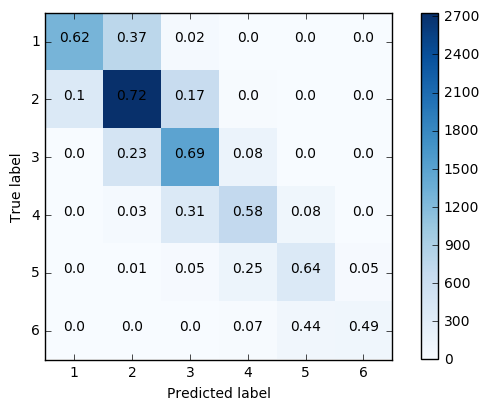
\includegraphics[width=.95\linewidth]{img/comb_d2_cm_favorites}
  \caption{Combined data set}
  \label{fig:d2_fav_distr_sub4}
\end{subfigure}%
\caption{Confusion matrices for multi-input deep neural networks}
\label{fig:d2_fav_cm}
\end{figure}
